%\section{Result}
\subsection{UNet++}
We trained UNet++ with the designated parameters, along with deep supervision and without supervision, which results in the accuracies in Table.\ref{tab:unetppResult}.

\begin{table}[!htbp]
\centering
\caption{UNet++ results}\label{tab:unetppResult}
\begin{tabular}{c|c|c|c|c}
\hline
& Out 1&Out 2&Out 3&Out 4\\    
\hline
with deep supervision & 0.878 & 0.886 & 0.891 & 0.894\\
without deep supervision & / & / & / & 0.917\\
\hline
\end{tabular}
\end{table}

As shown in Table.\ref{tab:unetppResult}, deep supervised network performance increases with output layer, while still performing worse than the network without deep supervision, where in the UNet++ paper\cite{unet_pp}, the gap was not that big, and deep-supervised network perform generally better than normal ones. We suppose that was caused by our non-ideal training parameter setting. We tend to think that deep-supervised networks actually converge slower in this setting because of two reasons:
\begin{itemize}
    \item Non-decaying deep supervision force the network to figure out a good approximation right at the beginning of the network, which may over-exploit the potential of the first layer, leaving less work to do for the following layers, and making the network less competent as a whole. We argue that this setup actually slows down the training process, which will be shown in the next experiment.
    \item Small training epochs lead to early exit and non-optimal performance during training.
\end{itemize}

\begin{figure}[!htpb]
\centering
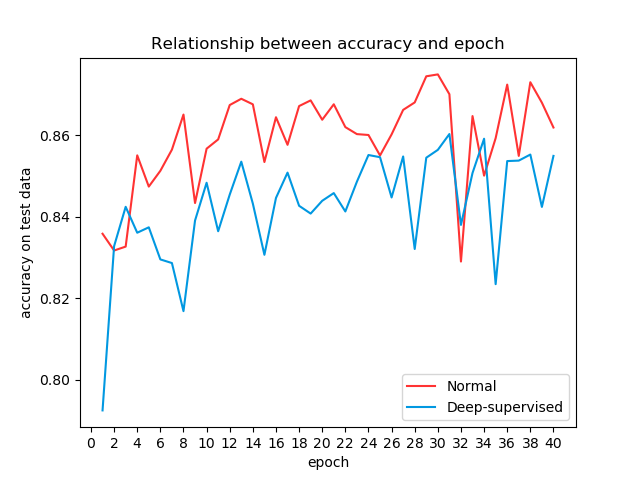
\includegraphics[scale=0.6]{figuras/unetppTraining.png}
\caption{UNet++ training accuracy-epoch curve.}
\label{fig:unetppTrain}
\end{figure}

As shown in Figure.\ref{fig:unetppTrain}, training accuracy of normal UNet++ are generally higher than deep-supervised UNet++, which is consistent with our former proposition. We can observe that the deep-supervised network, trained upon our poor laptop GPU with few epochs, could reach no better result than normal UNet++. We can conclude that deep supervision really slows down the training process. Although it may perform better in the end, it may take a much longer training time, which is still a problem for those who want to save the training calculation time.
